\section{Vortex Identification}
\label{ch:vortex}

Open from `3.\ Analysis $\to$ Vortex Identification`.

Vortex identification methods seek to objectively define the boundary and core of a vortex from the instantaneous or mean velocity field. \href{https://cmdrryder.github.io/uPrime/}{uPrime} implements five scalar criteria, which can be broadly divided into gradient-based (Eulerian) methods and the integral-based Graftieaux criteria.

\subsubsection*{Gradient-based methods}

All four gradient-based methods derive from the 2D velocity gradient tensor:
\[
\nabla \mathbf{u} = \begin{pmatrix} \partial u/\partial x & \partial u/\partial y \\ \partial v/\partial x & \partial v/\partial y \end{pmatrix}
\]
which is decomposed into its symmetric strain rate $\mathbf{S} = \tfrac{1}{2}(\nabla\mathbf{u} + \nabla\mathbf{u}^\top)$ and antisymmetric rotation rate $\boldsymbol{\Omega} = \tfrac{1}{2}(\nabla\mathbf{u} - \nabla\mathbf{u}^\top)$.

\begin{itemize}[leftmargin=1.5em]
  \item \textbf{Vorticity} $\omega = \partial v/\partial x - \partial u/\partial y$: the simplest measure of local rotation, but nonzero in shear layers even without a vortex core.

  \item \textbf{Q-criterion} (Hunt et al., 1988): $Q = -\tfrac{1}{2}(\partial_x u^2 + \partial_y v^2 + 2\,\partial_y u\,\partial_x v)$. A vortex core is identified where $Q > 0$, meaning rotation dominates strain. Q is the most widely used criterion in PIV literature.

  \item \textbf{Swirling strength} $\lambda_{ci}$ (Zhou et al., 1999): the imaginary part of the complex eigenvalue of $\nabla\mathbf{u}$. Complex eigenvalues exist only where the flow is locally swirling; $\lambda_{ci}$ is therefore immune to pure shear contamination that inflates $\omega$ and $Q$ in shear layers. \href{https://cmdrryder.github.io/uPrime/}{uPrime} multiplies by $\text{sign}(\omega)$ to retain rotation direction.

  \item \textbf{$\lambda_2$-criterion} (Jeong \& Hussain, 1995): identifies a vortex core as a connected region where the second eigenvalue of $\mathbf{S}^2 + \boldsymbol{\Omega}^2$ is negative. This criterion has a direct physical motivation: $\lambda_2 < 0$ marks regions where the centrifugal tendency of the pressure field overcomes both strain and unsteady effects.
\end{itemize}

\noindent\textbf{References:} Hunt, J.C.R., Wray, A. \& Moin, P. (1988). Eddies, stream, and convergence zones in turbulent flows. \textit{CTR Report CTR-S88}, 193--208. Zhou, J., Adrian, R.J., Balachandar, S. \& Kendall, T.M. (1999). Mechanisms for generating coherent packets of hairpin vortices in channel flow. \textit{Journal of Fluid Mechanics}, 387, 353--396. Jeong, J. \& Hussain, F. (1995). On the identification of a vortex. \textit{Journal of Fluid Mechanics}, 285, 69--94.

\subsubsection*{Graftieaux $\Gamma$ functions}

The $\Gamma$ functions (Graftieaux et al., 2001) are computed directly from the velocity vectors without differentiation, making them substantially more robust to PIV measurement noise:
\[
\Gamma_1(P) = \frac{1}{N} \sum_{M \in \mathcal{S}} \sin\!\left(\widehat{\mathbf{PM},\, \mathbf{U}_M}\right), \qquad
\Gamma_2(P) = \frac{1}{N} \sum_{M \in \mathcal{S}} \sin\!\left(\widehat{\mathbf{PM},\, \mathbf{U}_M - \widetilde{\mathbf{U}}}\right)
\]
where $\mathcal{S}$ is a local neighborhood of $N$ points around $P$, $\widehat{(\cdot,\cdot)}$ denotes the angle between two vectors, and $\widetilde{\mathbf{U}}$ is the local mean velocity over $\mathcal{S}$. Both functions are bounded between $-1$ and $+1$. The sign gives the rotation direction ($+1$ = CCW, $-1$ = CW). A vortex \emph{core} is identified where $|\Gamma_1| > 0.6$--$0.7$; the vortex \emph{boundary} is where $|\Gamma_2| > 2/\pi \approx 0.64$. The neighborhood half-width $S$ (default 2, corresponding to a $5 \times 5$ stencil) is user-adjustable.

\noindent\textbf{Reference:} Graftieaux, L., Michard, M. \& Grosjean, N. (2001). Combining PIV, POD and vortex identification algorithms for the study of unsteady turbulent swirling flows. \textit{Measurement Science and Technology}, 12(9), 1422--1429.

\subsection{Field View tab}

```{note}
\begin{enumerate}[leftmargin=1.5em, topsep=2pt]
  \item Select the scalar field and input (mean or instantaneous frame).
  \item Click `Compute Field`.
  \item Set the threshold fraction and sign filter, then click `Detect Vortices`.
  \item Check `Show vortex boundaries` to overlay detected contours on the colormap.
\end{enumerate}
```

The threshold is expressed as a fraction of the field maximum, making it dataset-agnostic. The actual physical value is shown in the readout next to the slider. For the $\Gamma$ criteria the threshold has a universal meaning ($|\Gamma_1| = 0.6$ corresponds to the standard core boundary); for gradient-based criteria it is dataset-dependent and must be chosen by the user.

\begin{figure}[htbp]
  \centering
  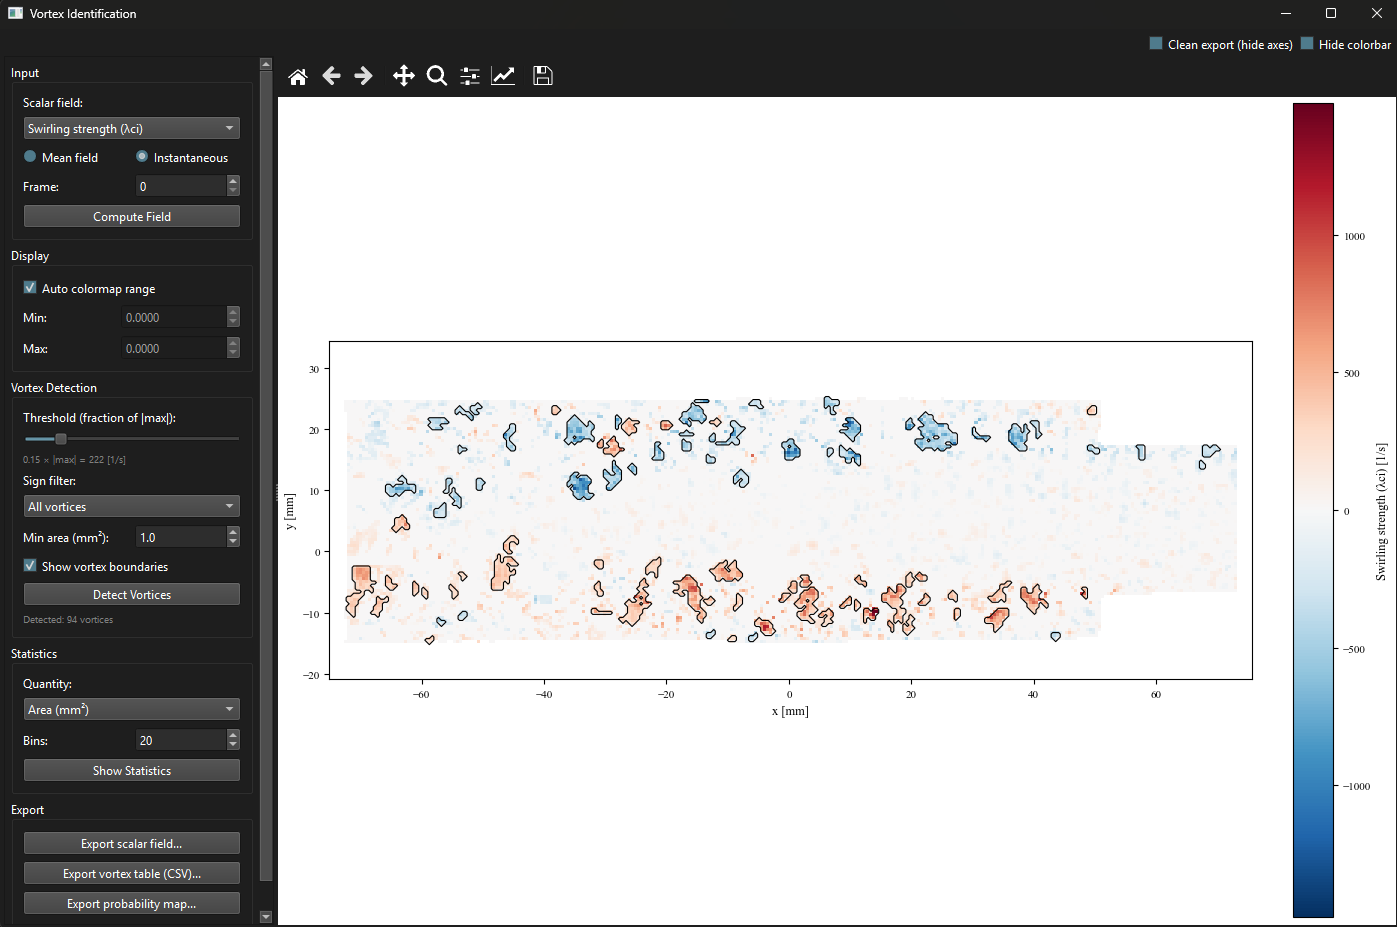
\includegraphics[width=0.92\linewidth]{fig_vortex_field}
  \caption{Vortex Identification window showing the swirling strength $\lambda_{ci}$ field for an instantaneous snapshot. Detected vortex boundaries (black contour lines) are overlaid on the colormap. The threshold is set to 15\% of the field maximum. Red regions indicate positive (CCW) rotation; blue regions indicate negative (CW) rotation. A total of 94 vortices are detected above the minimum area threshold.}
  \label{fig:vortex_field}
\end{figure}

```{tip}
For PIV data, start with $\Gamma_1/\Gamma_2$, which is most robust to measurement noise. Cross-check with Q-criterion or $\lambda_{ci}$. If the two methods agree, the detected structures are reliable.
```

\subsection{Vortex Statistics tab}

After clicking `Show Statistics`, two plots appear: a spatial probability map showing how often a vortex is detected at each grid point across all snapshots, and a histogram of the selected per-vortex quantity (area, circulation, or aspect ratio) with positive and negative vortices shown separately in red and blue.

\begin{figure}[htbp]
  \centering
  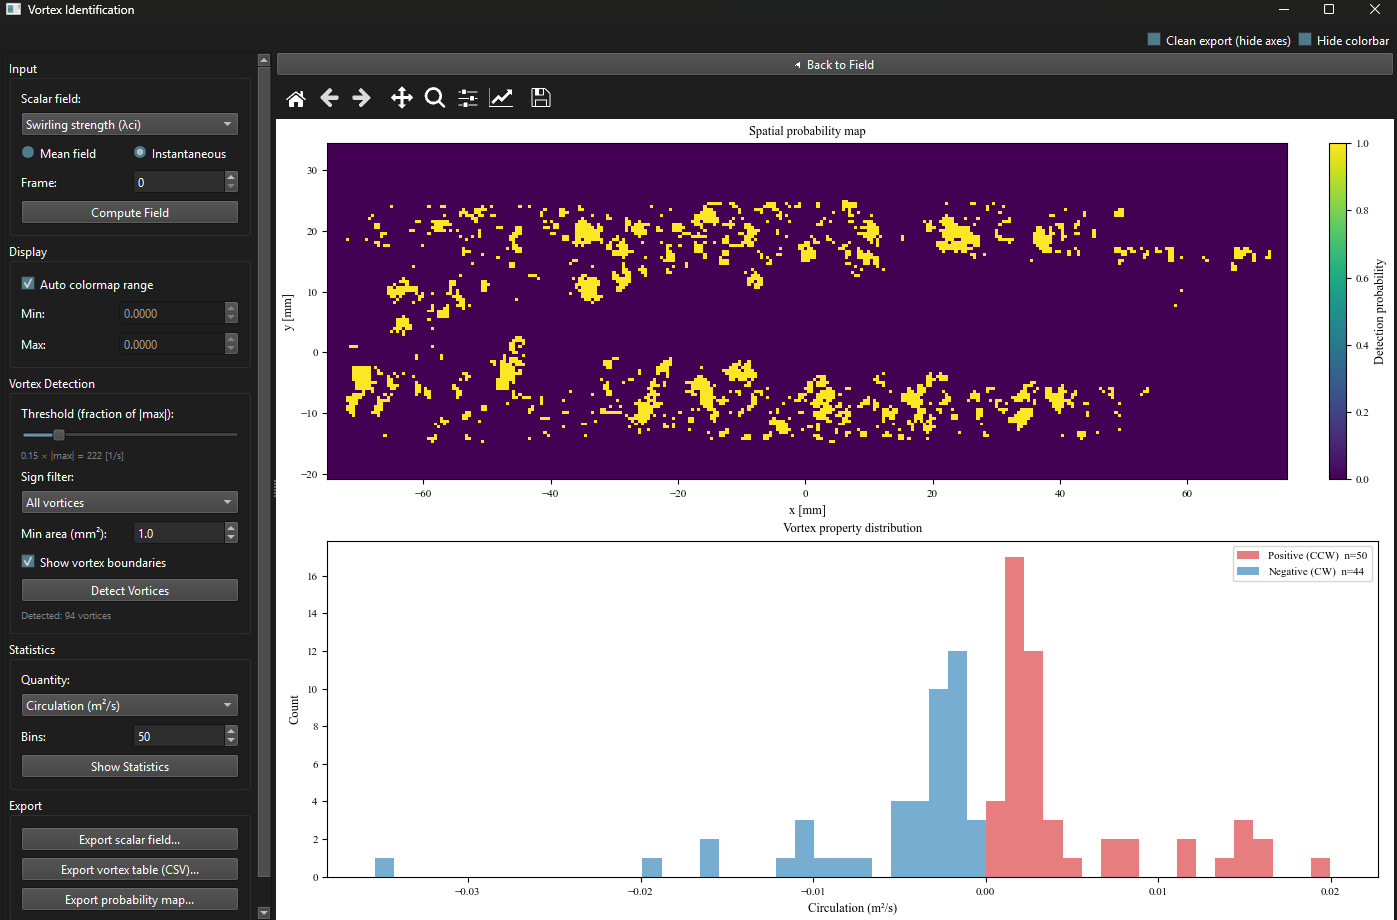
\includegraphics[width=0.92\linewidth]{fig_vortex_stats}
  \caption{Vortex Statistics view. Top: spatial probability map showing the fraction of snapshots in which a vortex is detected at each grid point (viridis colormap, 0--1). Yellow regions indicate persistent vortex locations concentrated in the shear layers. Bottom: circulation histogram for 94 detected vortices (50 CCW in red, 44 CW in blue). The near-symmetric distribution about zero is consistent with a turbulent shear layer with no mean rotation bias.}
  \label{fig:vortex_stats}
\end{figure}

\subsection{Exporting}

Click `Export scalar field\ldots` to save the scalar field as a Tecplot \texttt{.dat} file. Click `Export vortex table (CSV)\ldots` to save a per-vortex table with columns: vortex ID, centroid position, area, sign, circulation, aspect ratio, and frame index. The default filename now reflects the active criterion (e.g.\ \texttt{vortex\_lambda\_ci\_dataset.csv}). This CSV is designed to be imported into post-processing scripts for vortex tracking or further statistical analysis.

% ============================= CHAPTER 13 ==============================
